\documentclass[10pt,a4paper]{article}
\usepackage[english]{babel}
\usepackage{amsmath}
\usepackage{amsfonts}
\usepackage{amssymb}
\usepackage{tikz}
\usepackage{float}
\usepackage{graphicx}
\usetikzlibrary{shapes,shadows,arrows, positioning}
\bibliographystyle{plain}
\tikzstyle{entity}=[rectangle, draw=black, rounded corners, fill=blue!40, drop shadow, anchor=north, text=white,text width=10em, minimum width=2.7cm]
\tikzstyle{line} = [draw, -latex']
\tikzstyle{block} = [rectangle, draw, fill=blue!20, 
    text width=7em, text centered, rounded corners, minimum height=4em]
\tikzstyle{inblock} = [rectangle, draw, fill=green!30, 
    text width=7em, text centered, rounded corners, minimum height=4em]
\tikzstyle{exblock} = [rectangle, draw, fill=red!30, 
    text width=7em, text centered, rounded corners, minimum height=4em]
\tikzstyle{border1} = [rectangle, fill=white!100, ultra thick, draw=black!80,
            minimum height=60mm, minimum width=12cm,outer sep=0pt]
\tikzstyle{border2} = [rectangle, fill=white!100, ultra thick, draw=black!80,
            minimum height=8cm, minimum width=10cm,outer sep=0pt]            
\tikzstyle{border3} = [rectangle, fill=white!100, ultra thick, draw=black!80,
            minimum height=10cm, minimum width=13cm,outer sep=0pt]  
\author{P. J. G. Jordaan \\
15660796 \\
Department of Computer Science \\
University of Stellenbosch}
\title{Minke: Crowdsourced Price-tracking}
\date{}
\begin{document}
\maketitle
\pagebreak
\section{Introduction}
The Crowdsourced Price-tracking project focuses on bringing users accurate and relevant information about groceries and stores in order to give them the cheapest and closest options available. I aim to achieve this by combining web and mobile technology to create a simple, yet powerful shopping assistant.

\section{Problem Description}

This project wishes to answer the following question:
How can we best provide people with accurate and up-to-date information about wide spectrum of products at a variety of locations?
In particular we wish to provide this sort of information in both a mobile and a web format about grocery shopping at supermarkets. 
Furthermore we will need to get users to provide us with data for the system via a mobile application.

\section{Current Solutions}

There are a number of mobile applications available which are used to improve users's shopping experience. Many of these use bar code scanning to fetch product information, however most of them don't work in South Africa. Some of the current solutions are:
\begin{description}
\item[Google Shopper~\cite{google}] Google's take on a shopping assistant. This app provides:
\begin{itemize}
\item Bar code scanning of products to obtain information about them.
\item Scanning of a CD, DVD, book or video game's cover art to obtain information about it.
\item Voice search for products.
\item Price comparison
\item View nearby offers via Google Places.
\item Save your history, create favourites.
\item Share deals using social media.
\item View nearby stores and directions.
\item Not currently available in South Africa.
\item No web implementation.
\end{itemize}
\item[Barcode Scanner~\cite{scanner}] A very popular bar code scanner. It :
\begin{itemize}
\item Uses open source bar code processing Java library (ZXing).
\item Uses Google Product Search and Google Web Search to find information about bar codes.
\item No web implementation.
\end{itemize}
\item[ShopSavvy~\cite{shopsavvy}] The leader in mobile shopping provides the following :
\begin{itemize}
\item Uses bar code scanning and normal searching.
\item Allows users to make purchases from within app.
\item Allows users to create new products for unidentified items.
\item Provides information about deals, e.g. coupons and weekend sales.
\item No web implementation.
\item Not currently available in South Africa.
\end{itemize}
\item[PriceCheck~\cite{pricecheck}] A South African price comparison site and app. It provides the following:
\begin{itemize}
\item Price comparison.
\item Uses bar code scanning, normal searching and browsing.
\item Online searching, browsing and shopping as well.
\item Only recently started integrating grocery shopping.
\item Around since 2006, owned by Naspers.
\item Provides user registration and favourites.
\item Product and retailer rereviews.
\item Available on Android, iOS and Blackberry.
\end{itemize}
\end{description}
It is clear that although there are currently solutions which approach our problem, most of them quite match up to what we want to do, mostly due to lacking support in South Africa or lacking web support. PriceCheck is the only current solution that can be considered a direct competitor and it has only recently branched into grocery shopping with most of its focus lying elsewhere.

\section{Design}
The system will be known as Minke after the baleen whale.
\subsection{Goals}
Before the actual design of the system, I set out the following goals that I had in mind for the finished product:
\begin{description}
\item [Simplicity] The system must be intuitive and easy to use; no real explanations should be required for any aspects of the system. 
\item [Speed] The response time of the system for any user actions should be very quick since this system will typically be used in a situation where the user has no time to waste. 
\item [Elegance] A clean, elegant, uncluttered interface is a must. Only put what is needed on the interface.  
\item [Accuracy] We do want accurate results for the users, although this must not come at the cost of one of the other goals.
\item [Integration] The two user components of the system must blend together seamlessly. If a user can use one component they will also feel completely at home using the other. 
\end{description}

\subsection{Technology}

There are various parts of the system where what technology we will use will play a major role in how our system will work. Our chosen technology for developing the web application is Google Web Toolkit (GWT)~\cite{gwt}. This is due to the fact that it works well with Google App Engine (GAE)~\cite{gae} and tt also allows the developer to write mostly native Java code without having to resort to JavaScript or too much HTML. This eliminates the need to learn a new language since the developer is already familiar with Java and has experience with GWT. \\
GAE is a platform as a service (PaaS) cloud computing platform which allows users to develop and host applications in a Google data center. GAE provides amongst other services, a Datastore API which we will use to store our application's data which can then be accessed by both our mobile and our web applications. It also provides us with free hosting for our web application, which should be sufficient to fit to the needs of our application. The Datastore was chosen over Cloud SQL due to the billing which was introduced for Cloud SQL~\cite{cloud}. \\
The mobile application is to be developed only for Android~\cite{android}, with minimum compatibility with Android 2.3 Gingerbread. This is done for a number of reasons:
\begin{itemize}
  \item Coding can be done mostly in Java.
  \item By choosing Gingerbread as our minimum version, we accomodate upwards of 80\% of Android users.
  \item The developer has some experience with Android development.
\end{itemize}
Our mobile application will interact with the Datastore via HTTP requests with JavaScript Object Notation (JSON) used to send data. The reasons for this choice are:
\begin{itemize}
  \item Google's Android Cloud to Device Messaging (C2DM) service has been deprecated.
  \item Google Cloud Messaging (GCM) is still in an experimental stage.
  \item It easy to parse and build JSON data, especially for entities in a database.
  \item JSON offers lower overheads than other formats such as XML.
\end{itemize}
In terms of scanning products, there are two routes available to us: Optical Character Recognition (OCR) or Bar Code Scanning (BCS). OCR will work by having the user scan in a products entire price tag. This has the advantage that it will scan the price along with the product's identifier. However not all products have a price tag attached which does not make this an entirely viable option. Furthermore it seems that the only available open source implementation of OCR is Google's Tesseract OCR engine~\cite{tesseract}. Unfortunately this is written in C++ which makes it difficult to use with an Android app (which is coded in Java). It is however possible to use it within an Android app, via the Android NDK. \\
Our other option, BCS, seems to work very well in Android with most recognition software making use thereof. Since nearly every product should have a bar code attached, this guarantees that customers will be able to scan their products. The drawback is that customers would have to fill in the price of the product after it is scanned, but with a good interface this should take no longer than a second or two. The best open source library available to do bar code scanning with is ZXing~\cite{zxing} which is responsible for the aforementioned Barcode Scanner. This provides integration with their Barcode Scanner or allows you to build your own. It seems clear that BCS is the way to go since it is far simpler to implement, will scan all products and it has an established working app.

\subsection{System Features}
After looking at the currently used solutions, as well as our particular problem, the following features have been chosen to be included in our system:
\begin{itemize}
\item Provides online and mobile searching and browsing.
\item Android app uses BCS to identify our product.  
\item Allows users to create new products for unidentified items.
\item Allows users to update existing products prices.
\item Allows users to create new stores and towns.
\item Allows users to view nearby stores and directions.
\item Allows users to compare product prices.
\item Chart visualization of product price histories (mobile and online).
\item Allows users to find cheapest stores which stock their shopping list.
  \item View a store or product's location on a map as well as directions to it.
\end{itemize}

\subsection{System Components}
The Minke system will consist of three major components: A GWT web-side front-end, a GAE Datastore back-end and an Android mobile application. 
The GWT component will provide a web front-end for users to view information about product price histories and determine the best location to do their shopping at. Admin users will also be able to edit data on this platform. The Android application will be the primary source of data for the system and will rely on users scanning product tags at various stores. GAE will provide our web application's hosting and a Datastore for the entire system.
\tikzstyle{small} = [rectangle, fill=white!100, ultra thick, draw=black!80,
            minimum height=5cm, minimum width=8cm,outer sep=0pt] 
\begin{center}
\begin{figure}[H]
\pgfdeclarelayer{background}
\pgfsetlayers{background,main}
\begin{tikzpicture}[node distance=2cm]
\begin{pgfonlayer}{background}
        \node [small] (small) at (0,-2.5){};
    \end{pgfonlayer}
    \node (minke) [block]
        {
            \textbf{Minke}\\
            Crowdsourced Price-tracker
        };
        \node (GAE) [block, below of= minke]
        {
            \textbf{GAE}\\
            Datastore back-end
        };
    \node (GWT) [block, below left= 0.5cm and -0.3cm of GAE]
        {
            \textbf{GWT}\\
            Web front-end
        };
        \node (android) [block,below right= 0.5cm and -0.3cm of GAE]
        {
            \textbf{Android}\\
            Mobile front-end
        };
    
     \path [line] (GAE) -- (GWT);
    \path [line] (GWT) -- (GAE);
     \path [line] (GAE) -- (android);
     \path [line] (android) -- (GAE);
 \end{tikzpicture}
  \caption{High-level view of the Minke System.}
 \end{figure}
\end{center}


\subsection{GAE}

The Datastore back-end will store data about products as well as the locations the products were scanned at. 
Objectify-Appengine~\cite{ofy} will be used to provide a convenience layer between the Plain Old Java Objects (POJOs) used in our GWT system and the GAE Datastore API. This was due to the following reasons:
\begin{itemize}
\item You can persist, retrieve, delete, and query your own typed objects.
\item It allows all native Datastore features (batch operations, queries, entity groups, asynchronous operations, and partial indexes).
\item It provides type-safe key and query classes using generics.
\item Easy-to-use query interface.
\item Fast start-up.
\item Supports caching of data for fast read performance.
\item Use with GWT with no need for Data Transfer Objects (DTOs).
\item No external dependencies, only need GAE SDK.
\end{itemize}
GWT client access to the Datastore will be done via Remote Procedure Calls (RPCs) which will asynchronously update the client's data. Android access will be done via HTTP requests with JSON used to send data. 
\tikzstyle{small} = [rectangle, fill=white!100, ultra thick, draw=black!80,
            minimum height=3cm, minimum width=8cm,outer sep=0pt] 
\begin{center}
\begin{figure}[H]
\pgfdeclarelayer{background}
\pgfsetlayers{background,main}
\begin{tikzpicture}[node distance=2cm]
\begin{pgfonlayer}{background}
        \node [small] (small) at (0,-1.5){};
    \end{pgfonlayer}
        \node (GAE) [block]
        {
            \textbf{GAE \\
            Datastore back-end}
        };
        \node (nodey) [text width=4cm, below of= GAE]{};
        \node (product) [block, left of= nodey]
        {
            \textbf{Product Entities}
        };
        \node (location) [block, right of= nodey]
        {
            \textbf{Location Entities}
        };
     \path [line] (product) -- (location);
     \path [line] (location) -- (product);
 \end{tikzpicture}
  \caption{GAE Datastore back-end.}
 \end{figure}
\end{center}


\subsection{GWT}
The GWT component will consist of the following components:
\begin{description}
\item[Product Browser] This will allow the user to browse for products and view information about them.
\item[Shopping List Browser] This will allow the user to enter a shopping list and view the various locations they can do  their shopping at.
\item[Directions Viewer] This will the user to view directions to a store in the form of instructions as well as a map.
\item[Product Graph Viewer] This will allow the user to view product price histories in the form of a chart.
\item[Admin Viewer] This will allow administrators to edit dirty data.
\end{description} 
\tikzstyle{small} = [rectangle, fill=white!100, ultra thick, draw=black!80,
            minimum height=5cm, minimum width=10cm,outer sep=0pt] 
\begin{center}
\begin{figure}[H]
\pgfdeclarelayer{background}
\pgfsetlayers{background,main}
\begin{tikzpicture}[node distance=3cm]
\begin{pgfonlayer}{background}
        \node [small] (small) at (0,-2.5){};
    \end{pgfonlayer}
    \node (GWT) [block]
        {
            \textbf{GWT}\\
            Web front-end
        };
        \node (shopping) [block, below=0.5cm of GWT]
        {
            \textbf{Shopping List Browser}
        };
        \node (product) [block, left of= shopping]
        {
            \textbf{Product Browser}
        };
         \node (admin) [block, right of= shopping]
        {
            \textbf{Admin Viewer}
        };
        \node (directions) [block, below=0.5cm of product]
        {
            \textbf{Directions Display}
        };
        \node (graph) [block, below=0.5cm of shopping]
        {
            \textbf{Product Graph Viewer}
        };
    
     \path [line] (product) -- (graph);
     \path [line] (shopping) -- (directions);
     \path [line] (shopping) -- (graph);
 \end{tikzpicture}
  \caption{High-level view of GWT Web front-end.}
 \end{figure}
\end{center}

\subsubsection{Product Browser}

The Product Browser will consist of the following components:
\begin{description}
\item[Product Search] This will allow the user search for products by name,
category and location. The results of this will be displayed in the Product Viewer.
\item[Product Viewer] This will present the user with a tabular display of the products they searched for.
 The display will also contain links to the Info Popup and the Graph Chooser.
\item[Info Popup] This will display extra information about a chosen product.
\item[Graph Chooser] This will allow the user choose the number of products they wish to have displayed. This will then take the user to the Graph Viewer.
\end{description} 
\input{gwt-pb-diag}

\subsubsection{Shopping List Browser}

The Shopping List Browser will consist of the following components:

\begin{description}
\item[Shopping List Creator] This will allow the user to enter a shopping list of their choosing. The system will then determine all stores which stock the products as well as the total cost of the shopping list at each store. The results of this will be displayed in the Store Viewer.
\item[Store Viewer] This will present the user with a tabular display of the stores which stock the products in their shopping list. The display will also contain a link to the Shopping List Viewer and the Directions Viewer for each store.
\item[Shopping List Viewer] This will display extra information about the shopping list for the chosen store.
\end{description} 
\input{gwt-sl-diag}

\subsubsection{Admin Viewer}

The Admin Viewer will consist of the following components:

\begin{description}
\item[Entity Chooser] This will choose an entity type to view. The results of this will be displayed in the Entity Viewer.
\item[Entity Viewer] This will present the user with a tabular display of the entities and their fields. The display will also contain a link to the Entity Editor for each entity.
\item[Entity Editor] This will allow a user to edit an entities fields or to delete an entity entirely.
\end{description} 
\input{gwt-av-diag}

\subsubsection{Graph Viewer}

The Graph Viewer will consist of a single chart which will display a line plot of date against price for the chosen products. A scatter plot will be used if the number of data points becomes to high for the line plot to present a good visual display. Google's GWT Visualization API~\cite{viz} will be used to create the graph.
\input{gwt-gv-diag}

\subsubsection{Directions Viewer}

The Directions Viewer will consist of a Directions Display and a Map Display. The  Directions Display will be a textual
description of how to arrive at a given location from the user's location. The Map Display will relay this same information on a map. Google's GWT Maps API~\cite{gmaps} will be used to create the map and display the directions.

\input{gwt-dv-diag}


\subsection{Android}

The Android subsystem will consist of the following components:
\begin{description}
\item [Product Scanner] This allows the user to scan in a product's bar code and view information about it.
\item[Product Browser] This will allow the user to browse for products and view information about them.
\item[Shopping List Browser] This will allow the user to enter a shopping list and view the various locations they can do  their shopping at.
\item[Directions Viewer] This will the user to view directions to a store in the form of instructions as well as a map.
\item[Product Graph Viewer] This will allow the user to view product price histories in the form of a chart.
\end{description} 
\tikzstyle{small} = [rectangle, fill=white!100, ultra thick, draw=black!80,
            minimum height=6cm, minimum width=10cm,outer sep=0pt] 
\begin{center}
\begin{figure}[H]
\pgfdeclarelayer{background}
\pgfsetlayers{background,main}
\begin{tikzpicture}[node distance=3cm]
\begin{pgfonlayer}{background}
        \node [small] (small) at (0,-3){};
    \end{pgfonlayer}
    \node (Android) [block]
        {
            \textbf{Android}\\
            Mobile front-end
        };
        \node (scanner) [block, below=0.7cm of Android]
        {
            \textbf{Product Scanner}
        };
        \node (product) [block, left of= scanner]
        {
            \textbf{Product Browser}
        };
        \node (shopping) [block, right of= scanner]
        {
            \textbf{Shopping List Browser}
        };
        \node (directions) [block, below of= product]
        {
            \textbf{Directions Display}
        };
        \node (graph) [block, below of= shopping]
        {
            \textbf{Product Graph Viewer}
        };
     \path [line] (scanner) -- (product);   
     \path [line] (product) -- (graph);
      \path [line] (product) -- (directions);
     \path [line] (shopping) -- (directions);
     \path [line] (shopping) -- (graph);
 \end{tikzpicture}
  \caption{High-level view of Android Mobile front-end.}
 \end{figure}
\end{center}

\subsubsection{Product Scanner}
\begin{description}
\item[Scan View] This will be the actual Barcode Scanner. Before scanning a user is prompted to choose the store they are at. If their store is not
available they are taken to the Store Creator. Otherwise BCS is loaded and scanning begins. The completed scan can have the following outcomes:
\begin{description}
  \item[Unsuccessful] User prompted to try again.
  \item[Not Found] User taken to Product Creator.
  \item[Found] User asked to update price and then taken to the Product Browser
  where they are shown the scanned product at all stores it has been scanned at. 
\end{description}
\item[Store Creator] This will allow the user to add a new store to the database. After this is done, a scan of a product begins.
\item[Product Creator] This will allow the user to add a new product to the database. After this is done, they are taken to the Product Browser.
\end{description} 
\input{and-ps-diag}

\subsubsection{Product Browser}

The Product Browser will function in the same fashion as the GWT Product Browser.

\subsubsection{Shopping List Browser}

The Shopping List Browser will function in the same fashion as the GWT Shopping List Browser.

\subsubsection{Graph Viewer}

The Graph Viewer will function in the same fashion as the GWT Graph Viewer. AChartEngine~\cite{achartengine} will be used  instead of the GWT Visualisation API.
\tikzstyle{small} = [rectangle, fill=white!100, ultra thick, draw=black!80,
            minimum height=3cm, minimum width=5cm,outer sep=0pt] 
\begin{center}
\begin{figure}[H]
\pgfdeclarelayer{background}
\pgfsetlayers{background,main}
\begin{tikzpicture}[node distance=2cm]
\begin{pgfonlayer}{background}
        \node [small] (small) at (0,-3.5){};
    \end{pgfonlayer}
      \node (nodex) [text width=4cm] {};
    \node (shop) [inblock, left of =nodex]
        {
            \textbf{Shopping List Browser}
        };
        \node (product) [inblock, right of= nodex]
        {
            \textbf{Product Browser}
        };
         \node(graph) [block, below of= nodex]
        {
            \textbf{Graph Viewer}
        };
        \node (viewer) [block, below of= graph]
        {
            \textbf{Graph Display}
        };
     \path [line] (product) -- (graph);
     \path [line] (shop) -- (graph);
     \path [line] (graph) -- (viewer);
 \end{tikzpicture}
  \caption{The Graph Viewer.}
 \end{figure}
\end{center}

\subsubsection{Directions Viewer}

The Directions Viewer will function in the same fashion as the GWT Directions Viewer. The library used for this will be the Google Maps API for Android~\cite{amaps}. Directions will be obtained from Google's Directions API via a HTTP request and using JSON to hold the data.
\tikzstyle{small} = [rectangle, fill=white!100, ultra thick, draw=black!80,
            minimum height=3cm, minimum width=7cm,outer sep=0pt] 
\begin{center}
\begin{figure}[H]
\pgfdeclarelayer{background}
\pgfsetlayers{background,main}
\begin{tikzpicture}[node distance=2cm]
\begin{pgfonlayer}{background}
        \node [small] (small) at (0,-3.5){};
    \end{pgfonlayer}
    \node (nodex) [text width=4cm] {};
    \node (shop) [inblock, left of =nodex]
        {
            \textbf{Shopping List Browser}
        };
        \node (product) [inblock, right of= nodex]
        {
            \textbf{Product Browser}
        };
        \node (viewer) [block, below of= nodex]
        {
            \textbf{Directions Viewer}
        };
        \node (nodey) [text width=4cm, below of= viewer]{};
        \node (directions) [block, right of= nodey]
        {
            \textbf{Directions Display}
        };
        \node (map) [block, left of= nodey]
        {
            \textbf{Map Display}
        };
     \path [line] (product) -- (viewer);
     \path [line] (shop) -- (viewer);
     \path [line] (viewer) -- (map);
     \path [line] (viewer) -- (directions);
 \end{tikzpicture}
  \caption{The Directions Viewer.}
 \end{figure}
\end{center}










\section{Implementation}
\subsection{GAE}
In order to understand how the system will function it is important to get an idea of how and what data will be stored.
Our entities within the Datastore are the following:
\begin{description}
\item [ProductCategory] Three nested categories associated with a product, e.g. Coffee Beans, Coffee, Consumables.
\item [Brand] Brand associated with a product, e.g. Jacobs.
\item[Product] A specific product, e.g. 500g Frisco.
\item[Country] A country, e.g. South Africa.
\item[Province] A province or state, e.g. Western Cape.
\item [City] A city or town, e.g. Stellenbosch.
\item [CityLocation] A GPS location together with its closest city.
\item [Store] A store franchise, e.g. Spar.
\item [Branch] A branch of a Store, e.g. Eikestad Woolworths.
\item [BranchProduct] The entity associated with a product at a specific branch.
\item [DatePrice] The price associated with a BranchProduct on a particular Date.
\end{description}
A clearer picture of the system is given in Figure 12.
\begin{center}
\begin{figure}[H]
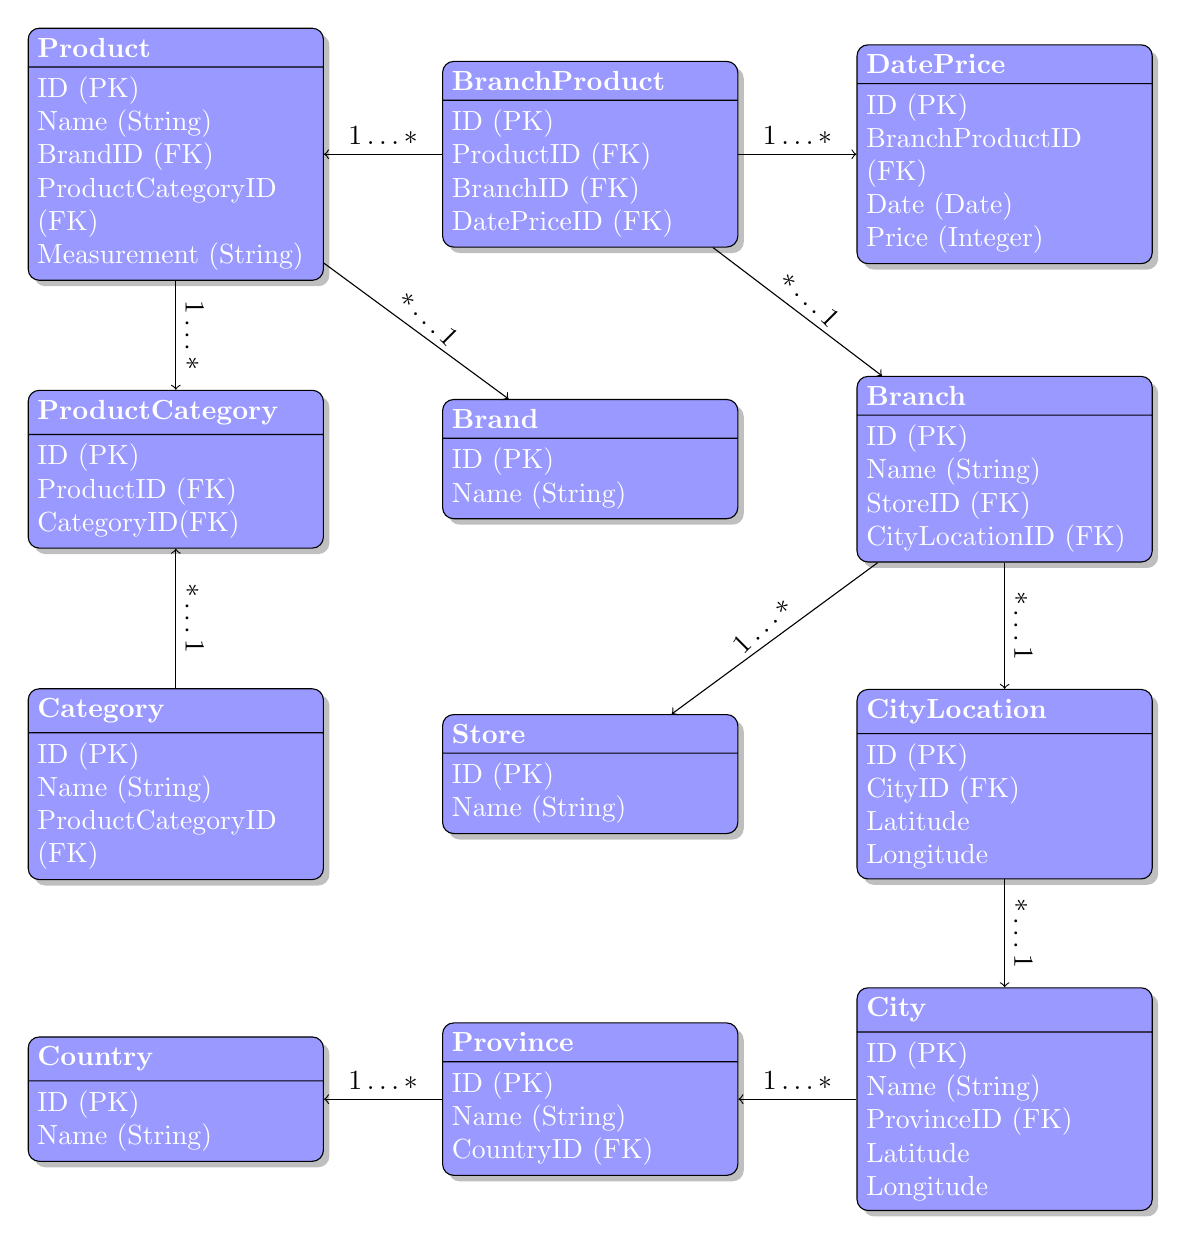
\begin{tikzpicture}[node distance=4cm]
    \node (bp) [entity, rectangle split, rectangle split parts=2]
        {
            \textbf{BranchProduct}\\
            \nodepart{second}ID (PK)\\
            ProductID (FK)\\
            BranchID (FK)\\
            DatePriceID (FK)\\
        };
         \node (dp) [entity, rectangle split, rectangle split parts=2, right=1.5cm of bp]
        {
            \textbf{DatePrice} \\
            \nodepart{second}ID (PK)\\
			  BranchProductID (FK)\\
			  Date (Date)\\
			  Price (Integer)\\
        };    
         \node (branch) [entity, rectangle split, rectangle split parts=2, below of= dp]
        {
            \textbf{Branch} \\
            \nodepart{second}ID (PK)\\
            Name (String)\\
			StoreID (FK)\\
			CityLocationID (FK)\\
        };
        \node (product) [entity, rectangle split, rectangle split parts=2, left=1.5cm of bp]
        {
            \textbf{Product} \\
            \nodepart{second}ID (PK)\\
            Name (String)\\
			      BrandID (FK) \\
			      ProductCategoryID (FK)\\
			      Measurement (String)\\
        };
        \node (brand) [entity, rectangle split, rectangle split parts=2, below right=1.5cm and 1.5cm of product]
        {
            \textbf{Brand} \\
            \nodepart{second}ID (PK)\\
            Name (String)\\
        };
        \node (store) [entity, rectangle split, rectangle split parts=2, below of=brand ]
        {
            \textbf{Store} \\
            \nodepart{second}ID (PK)\\
            Name (String)\\
        };

        \node (loc) [entity, rectangle split, rectangle split parts=2, below of= branch]
        {
            \textbf{CityLocation} \\
            \nodepart{second}ID (PK)\\
            CityID (FK)\\
            Latitude\\
            Longitude\\
        };
        \node (pc) [entity, rectangle split, rectangle split parts=2, below of= product]
        {
            \textbf{ProductCategory} \\
            \nodepart{second}ID (PK)\\
            ProductID (FK)\\
            CategoryID(FK)\\
        };
        \node (category) [entity, rectangle split, rectangle split parts=2, below of= pc]
        {
            \textbf{Category} \\
            \nodepart{second}ID (PK)\\
            Name (String)\\
            ProductCategoryID (FK)\\
        };
         \node (city) [entity, rectangle split, rectangle split parts=2, below of= loc]
        {
            \textbf{City} \\
            \nodepart{second}ID (PK)\\
            Name (String)\\
            ProvinceID (FK)\\
    		    Latitude\\
            Longitude\\
    	};
    	\node (province) [entity, rectangle split, rectangle split parts=2, left=1.5cm of city]
        {
            \textbf{Province} \\
            \nodepart{second}ID (PK)\\
            Name (String)\\
            CountryID (FK)\\
    	};
    	\node (country) [entity, rectangle split, rectangle split parts=2, left=1.5cm of province]
        {
            \textbf{Country} \\
            \nodepart{second}ID (PK)\\
            Name (String)\\
    	};
     \path[->] (bp) edge node[above] {$1 \ldots *$} (dp);
     \path[->] (bp) edge node[above] {$1 \ldots *$} (product);
     \path[->] (bp) edge node[above, rotate=-45] {$* \ldots 1$} (branch);
	 \path[->] (product) edge node[above, rotate=-90] {$1 \ldots *$} (pc);
	 \path[->] (product) edge node[above, rotate=-45] {$* \ldots 1$} (brand);
	 \path[->] (branch) edge node[above, rotate=45] {$1 \ldots *$} (store);
	 \path[->] (branch) edge node[above, rotate=-90] {$* \ldots 1$} (loc);
     \path[->] (loc) edge node[above, rotate=-90] {$* \ldots 1$} (city);
    \path[->] (city) edge node[above] {$1 \ldots *$} (province);
  \path[->] (province) edge node[above] {$1 \ldots *$} (country);
    \path[->] (category) edge node[above, rotate=-90] {$* \ldots 1$} (pc);
 \end{tikzpicture}
 \caption{Class Diagram of Entities used.}
 \end{figure}
\end{center}

The entities all have their own Data Access Objects (DAOs) which allow for querying, 
get and put operations. The DAOs are static objects which provide a simple interface for interacting with the
Objectify-AppEngine Datastore. They are all created when the system is loaded.
Each of the services used by the GWT front-end has an implementation on the GAE back-end. These are:
\begin{description}
\item[ClassService] Registers entities with Objectify. Also fetches a
particular class of entities, deletes or updates an entity for Admin Viewer.
\item[BranchProductService] Retrieves the following:
\begin{itemize}
\item BranchProducts which match a ProductCategory and/or a City or a Product.
\item Branches which stock a set of Products.
\item BranchProducts's price histories.
\end{itemize}
\item[ProductService] Retrieves all Products from the Datastore.
\item[CategoryService] Retrieves all Categories from the Datastore.
\item[LocationService] Retrieves all cities, countries or provinces from the
Datastore.
\end{description}

\subsection{GWT}
The GWT front-end has several central components which facilitate interaction between the subsystems described in Design.
In the *.client package we have:
\begin{description}
\item[WebSystem] The central system which:\begin{itemize}
\item Controls how the system interacts with GAE,
\item Requests data for and loads data into the Graphical User Interface (GUI),
\item Serves as the entry point for the system, and
\item Binds the different components together.
\end{itemize}  
\item[RPC] Responsible for interacting with the Datastore via RPCs. It provides the following services:  
\begin{itemize}
\item ClassService
\item BranchProductService
\item ProductService
\item ProductCategoryService
\item LocationService
\item GeoService : Determines user location using a GWT implementation of HTML5's GeoLocation~\cite{geo} interface.
\end{itemize}
 \item[SystemData] Stores data pulled from the Datastore.
\end{description}
 In the *.client.gui.* package we have:
 \begin{description}
  \item[WebPage] Holds the various GUI components. Facilitates interaction between GUI components.
  \item[ViewTree] Provides sidebar with shortcuts to each of the major components. 
  \item[button.*] Contains custom image buttons.
    \item[loader.Loader] A loader to be displayed when the system is busy.
    \item[popup.FocusedPopupPanel] A general purpose PopupPanel which disables the background when shown.
    \item[spinedit.SpinEdit] A SpinEdit (up and down button with an IntegerBox).
    \item[table.TableView] A general purpose table display created using a FlexTable.
\end{description}
 In the *.client.util package we have:
 \begin{description}
  \item[CSSUtils] Used to inject custom css styles.
  \item[GUIUtils] Provides static access to error dialogs and the loader.
    \item[ImageUtils] Provides easy access to images.
    \item[Utils] Provides some general methods needed by some of the GUI components.
\end{description}
\subsubsection{Product Browser}
The Product Browser was implemented as follows:
\begin{description}
\item[Product Search] This was implemented as ProductSearch, a PopupPanel which allows the user to 
search for products by name, category and location. This then sends the search request
 to the Datastore via WebPage, WebSystem and RPC and directs the user to
 ProductList.
 \item[Product Viewer]This was implemented as ProductList, which presents the
 user with a tabular display of the products they searched for. It contains buttons to access ProductDetail and GraphTypePopup.
\item[Info Popup] This was implemented as ProductDetail, a popup which displays
extra information about a chosen product.
\item[Graph Chooser] This was implemented as GraphTypePopup, a PopupPanel
which allows the user choose what type of chart they which to view, in terms of
which products they wish to have displayed. This will then take the user to
the Graph Viewer.
\end{description} 
\begin{figure}[h!]
\centering
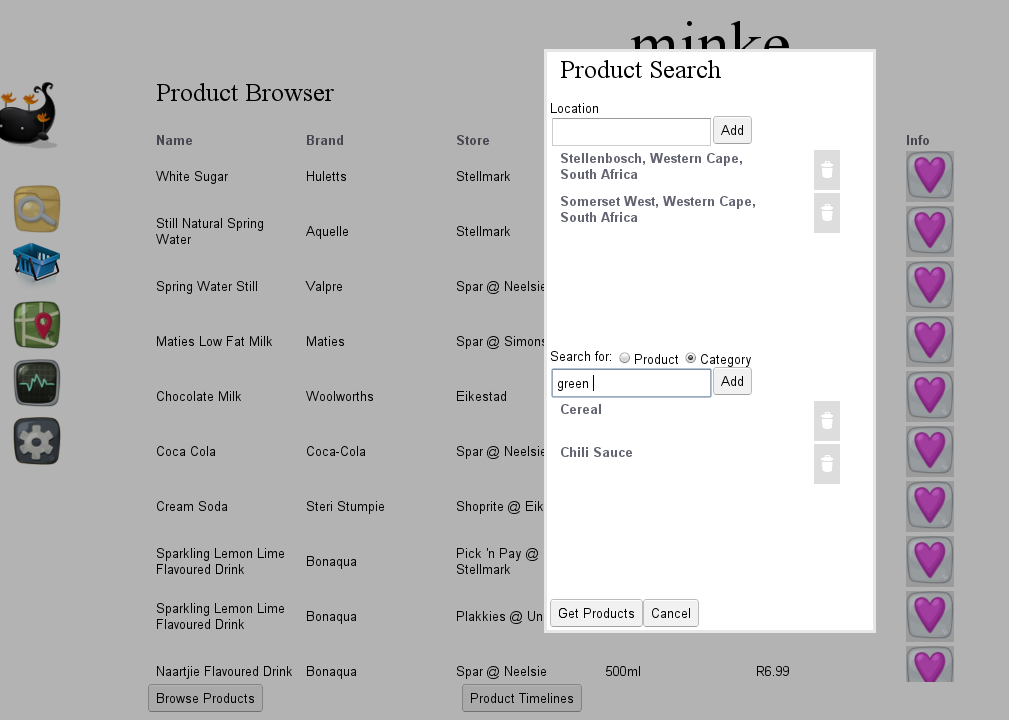
\includegraphics[width=0.8\textwidth]{gwt-search.png}
\caption{Product search interface with viewer in background.}
\end{figure}
\subsubsection{Shopping List Browser}
The Shopping List Browser was implemented using the following classes in the *.client.gui package:
\begin{description}
\item[popup.shoppinglist.ShoppingList] A popup which allows the user to add products to their shopping list via a SuggestBox~\cite{suggest}. This then sends the request for Branches which stock the products to the Datastore via WebPage, WebSystem and RPC.
\item[popup.shoppinglist.ShoppingListItem] A Composite~\cite{comp} GUI class used to represent a Product on the shopping list. Allows the user to adjust the quantity of a Product as well.
\item[table.BranchList] This presents the user with a tabular display of the Branches which stock the Products on their shopping list. This is created once the above RPC has successfully completed. It contains buttons to access ShoppingListDetail and the Directions Viewer.
\item[table.ShoppingListDetail] A table which displays the shopping list for a particular Branch. It therefore allows the user to see the price of each Product. It contains a button to access the Graph Viewer.
\item[popup.ShoppingListDetailPopup]A popup used to hold ShoppingListDetail.
\end{description}

\subsubsection{Admin Viewer}
A user is requested to enter a password before they are granted access to Admin
Viewer. The interface was implemented in the following manner:
\begin{description}
\item[Entity Chooser] This was implemented as EntityPopup, a PopupPanel with a
SuggestBox which allows the user to choose which type of entity to view. It
then requests it from the Datastore and directs the user to the DataViewer.
\item[Entity Viewer]This was implemented as DataViewer which provides the user
with a tabular view of all the entities of a particular type. It provides links
to EntityPopup and EditPopup.
\item[Entity Editor] This was implemented as EditPopup, a PopupPanel wich allows
a user to edit the various fields of a single entity or delete it completely.
After deleting or editing an entity, the DataViewer is updated with the new data
from the Datastore.
\end{description}
\begin{figure}[h!]
\centering
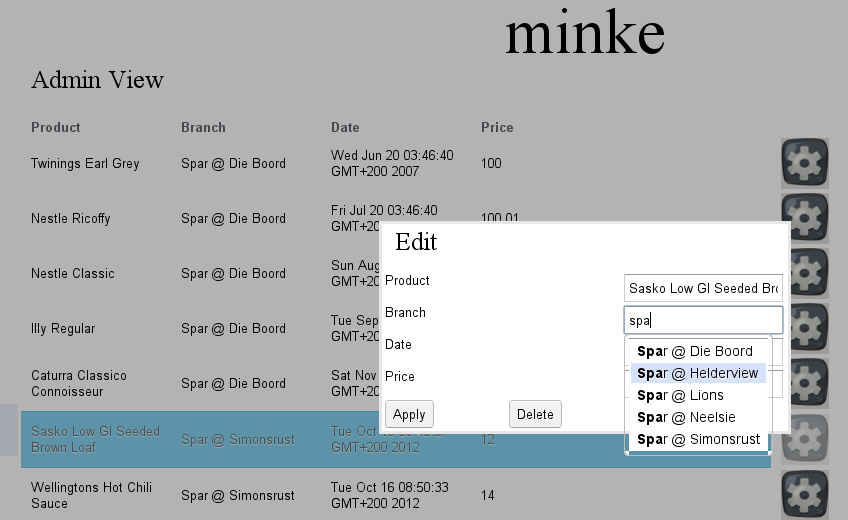
\includegraphics[width=0.8\textwidth]{gwt-admin.png}
\caption{The Entity Editor with Entity Viewer in the background.}
\end{figure}

\subsubsection{Graph Viewer}
The Graph Viewer was implemented in the following manner:
\begin{description}
\item[HistoryGraph] This was used to hold and display an instance of the
ScatterChart class as well as load the Visualization API. It also
provides a communication interface between ScatterGraph and the rest of the
system. It also allows data to be added to or removed from the current chart.
\item[ScatterGraph] A container for a ScatterChart~\cite{scatter} which loads a new chart when provided with data.
\end{description}
\begin{figure}[h!]
\centering
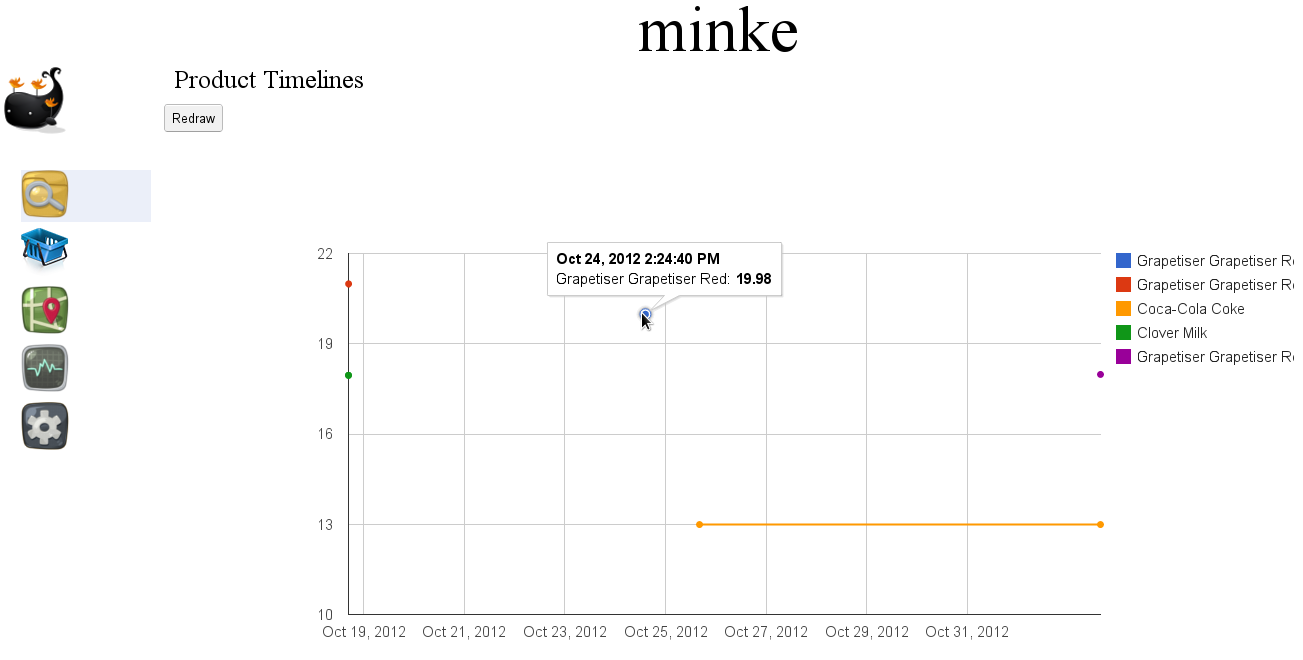
\includegraphics[width=1.0\textwidth]{gwt-graph.png}
\caption{The Graph Viewer interface.}
\end{figure}
\subsubsection{Directions Viewer}
The Directions Viewer was implemented using the following classes in the *.client.gui.map package:
\begin{description}
\item[BranchLocation] A container for the DirectionsMap class which also loads the Maps API. Also provides a communication interface between DirectionsMap and the rest of the system and allows the user to change their location.
\item[DirectionsMap] A container for a MapWidget~\cite{mwidget} and a DirectionsPanel~\cite{dpanel} which loads a new map and directions when provided with data in the form of a LatLng~\cite{latlng} map center and a String~\cite{string} containing an origin and a destination.
\end{description}


\subsection{Android}
The Android component of the system was implemented with the Android 4's design principles in mind. 
This means that the ActionBar has taken over the role traditionally occupied by the menu in previous versions of Android. 
Furthermore, emphasis has shifted away from Activity-centric to Fragment-oriented applications which allows for faster,
 more dynamic and interactive applications. With this in mind it was decided to
 implement the main section of our application as a single activity, called
 HomeActivity, which hosts different tabs for each main view (Product Scanner,
 Product Browser and Shopping List Browser) of our application.
 Each view would then be implemented as a series of Fragments which would move in and out of
 their respective tabs depending on the state of the view. The other views in
 our application (Graph View and Directions View) will be implemented as
 seperate activities which can be launched from our HomeActivity. Unfortunately
 much of this required functionality is not compatible with Android versions
 older than Honeycomb, therefore we needed a workaround. Fortunately this was
 available in the form of ActionBar Sherlock and androidv4, libraries which
 provide us with Android 4 functionality on older versions of Android.  
\subsubsection{Product Scanner}
Not yet implemented.

\subsubsection{Product Browser}
The Product Browser is found in the second tab in our HomeActivity. It was
implemented in the following manner:
\begin{description}
\item[Product Search] This was implemented in two seperate Fragments,
LocationSearchFragment and ProductSearchFragment. LocationSearchFragment allows
the user to specify the locations at which products must be searched for and is
the first Fragment to be displayed in the tab. Clicking on the search button in
it takes the user to the ProductSearchFragment which allows the user to specify
the products or categories to be searched for. Clicking on the search button
here initiates the actual search and takes the user to the BrowseFragment.
\item[Product Viewer] This was implemented as BrowseFragment which displays a
list of the found products. Each list item gives the product's name and price
and is clickable, with a click bringing up an Info Popup. There is also a graph
button present which takes the user to ChartActivity (described in Graph
Viewer).
\item[Info Popup] This was implemented an AlertDialog which displays
information about each product, including:
\begin{itemize}
  \item name,
  \item brand,
  \item size,
  \item price,
  \item date of last scan, and
  \item store scanned at.
\end{itemize} 
The dialog also allows the user to share the product using other applications or
to view the store the product was found at in MapsActivity (described in
Directions Viewer).
\end{description}
\begin{figure}[h!]
\centering
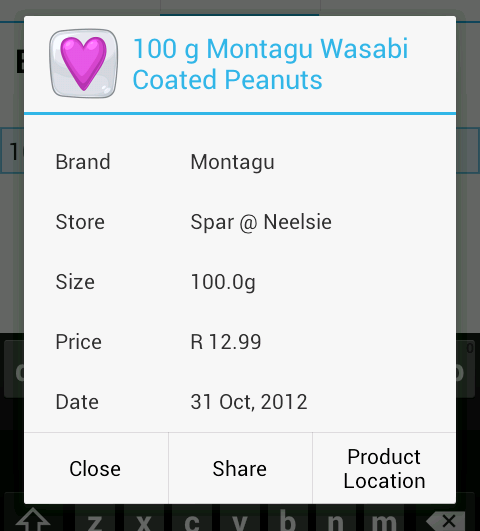
\includegraphics[width=0.3\textwidth]{product-info.png}
\caption{Product info display after a successful search.}
\end{figure}
\subsubsection{Shopping List Browser}
The Shopping List Browser is only partially implemented thus far, with only some of the GUI being designed.
These are the components which have been created:
\begin{description}
\item[ShopScreen] This presents users with a shopping list to which they can add Products.
\item[ShopListAdapter] This is used to display Products on the ShopScreen.
\end{description}

\subsubsection{Graph Viewer}
The Graph Viewer is partially implemented thus far using the following component:
\begin{description}
\item[GraphScreen] This presents users chart for a given dataset.
\end{description}

\subsubsection{Directions Viewer}
The Directions Viewer was implemented using MapsActivity to display our map
and directions in and GoogleParser to request directions from Google's
Directions API and parse so that they can be used in our application. Directions
are displayed in a dialog which can be accessed via a button on the ActionBar
and each intruction can be clicked on which will show the instruction on the
map. 
\begin{figure}[h!]
\centering
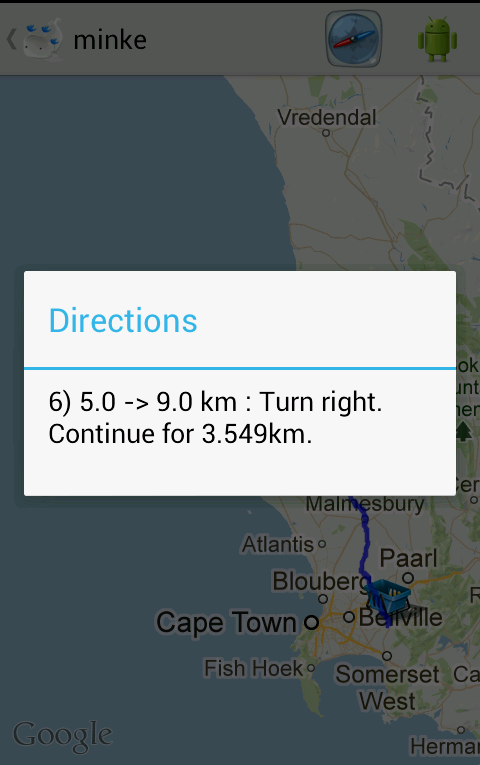
\includegraphics[width=0.3\textwidth]{directions.png}
\caption{Directions view with map.}
\end{figure}


\section{Conclusion}

Thus far I feel that the project has progressed well. The issues I have encountered were mostly due to a lack of experience with the tools that I chose to work. For example, initially the GUI of web application was badly written due to UiBinders not being used. This made the application slow and the interface clunky. The GAE Datastore was also switched to the Cloud SQL without conducting research into the billing which would be later be added to its use. So this led to the system having to be migrated back to the GAE Datastore.\\
The Web front-end prototype functions well with the App Engine Datastore. It is fast, responsive and easy-to-use. The Visualisation and Maps APIs blend into the application seamlessly. \\
The system now needs to be extended to fully integrate with the Android mobile application in order to allow the system to actually fulfil its intended function. \\
The main lesson that can be taken from the system thus far is that proper research, planning and design is essential. Furthermore scheduling for different stages of the project must be done well in advance in order to avoid rushing aspects thereof to meet deadlines.

\bibliography{report}

\end{document}
